\documentclass[a4paper,12pt]{article}
\usepackage{latexsym}
\usepackage{graphicx}
\usepackage{epsfig}
\usepackage{float}
\usepackage{natbib}
\usepackage{listings}
\graphicspath{{./}}
\DeclareGraphicsExtensions{.eps}
\author{Howard Kinsman}
\title{Cosmology Tutorial 1}
\begin{document}
\maketitle

\section{}
\begin{equation}
f=\frac{L}{4\pi r^2}
\end{equation}
and differentiating
\begin{equation}
\frac{df}{dr}=-\frac{L}{2\pi r^3}
\end{equation}
Number density = $\frac{1}{r}$ so
\begin{equation}
N=\frac{4}{3}\pi r^3 \times \frac{1}{r}
\end{equation}
\begin{equation}
N=\frac{4\pi r^2}{3}
\end{equation}
and differentiating
\begin{equation}
\frac{dN}{dr}=\frac{8\pi r}{L}
\end{equation}
dividing equation 5 by equation 2 gives
\begin{equation}
\frac{dN}{df}=\frac{-48\pi^2 r^4}{L}
\end{equation}
so that
\begin{equation}
\frac{dN}{df}\propto r^4
\end{equation}
$r^2\propto f^{-1}$ so that
\begin{equation}
\frac{dN}{df}\propto f^{-2}
\end{equation}
Therefore $\alpha = -2$. 
$dln f=\frac{1}{f}df$ so that
\begin{equation}
\mathcal{N}=\frac{dN}{dln f}=f\frac{dN}{df}
\end{equation}
which gives $\mathcal{N}\propto f^{-1}$ and so
\begin{equation}
log\mathcal{N}=-log f + const
\end{equation}
This is linear so measuring stellar fluxes would allow an observer to determine if the distribution was homogeneous.

\section{}
The NRAO VLA Sky Survey (NVSS) is a radio survey covering the sky north of -40° declination at 1.4GHz. It contains over a million 
rows so I extracted a subset of sources where the flux density $>100mJy$ giving appoximately 62,000 sources.

The Two Micron All Sky Survey (2MASS) Redshift Survey (2MRS) was a ten-year project to map the full three-dimensional distribution of galaxies in
the nearby universe. It provides a good census of baryonic matter in the nearby universe (to about 300 Mpc). It contains
about 400,000 rows so I only extracted sources with a magnitude $<13$ in the K band giving about 44,000 rows.

The 2MASS Extended Source Catalog (2MASX) contains over 1.6 millions rows and suveys the entire sky in the J, H and K bands.
I restricted the output to sources with a magnitude of $<13$ in the J band giving about 77,000 rows.

\section{}
Figure 1 shows a log of number counts per log flux for the NVSS. The slope was calculated:
\begin{equation}
\frac{log(2000/1000)}{log(100-200)}=-1
\end{equation}
This figure matches quite well with the figure of -1.5 calculated for a homogeneous universe. The slope is constant apart
from very small flux densities (probably due to sampling errors) and large flux densities (the universe is not
homogeneous on smaller scales).
\begin{figure}[H]
\centering
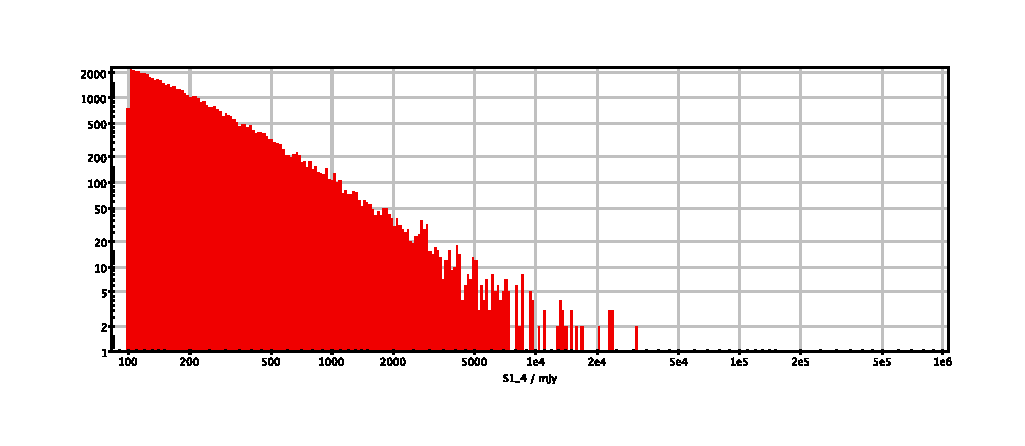
\includegraphics[width=.9\textwidth]{./NVSS.eps}
\caption{NVSS}
\label{fig:1}
\end{figure}
Figure 2 shows a log of number counts per magnitude in the K band for the 2MRS survey.
\begin{figure}[H]
\centering
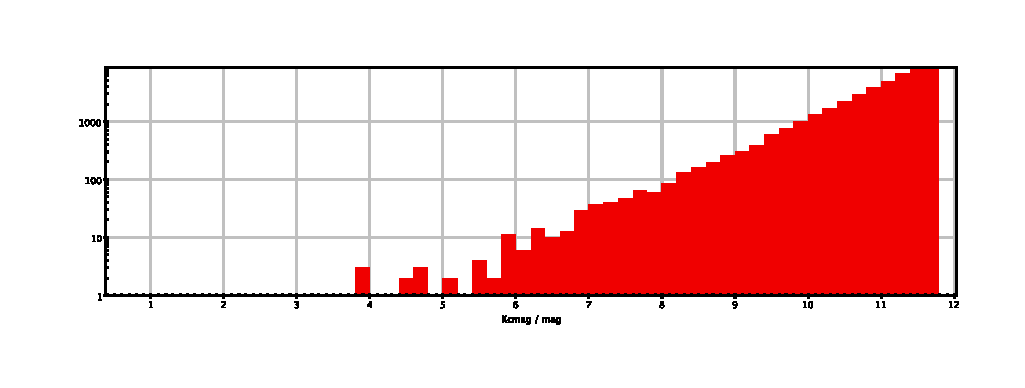
\includegraphics[width=.9\textwidth]{./2MRS.eps}
\caption{2MRS}
\label{fig:2}
\end{figure}
The slope was calculated as:
\begin{equation}
\frac{log(1000/100)}{10/7}=.8
\end{equation}
This also reasonably matches the expected slope of .6 for a homogeneous universe.
Finally figure 3 shows a log of number counts per magnitude in the J band for the 2MASX survey.
\begin{figure}[H]
\centering
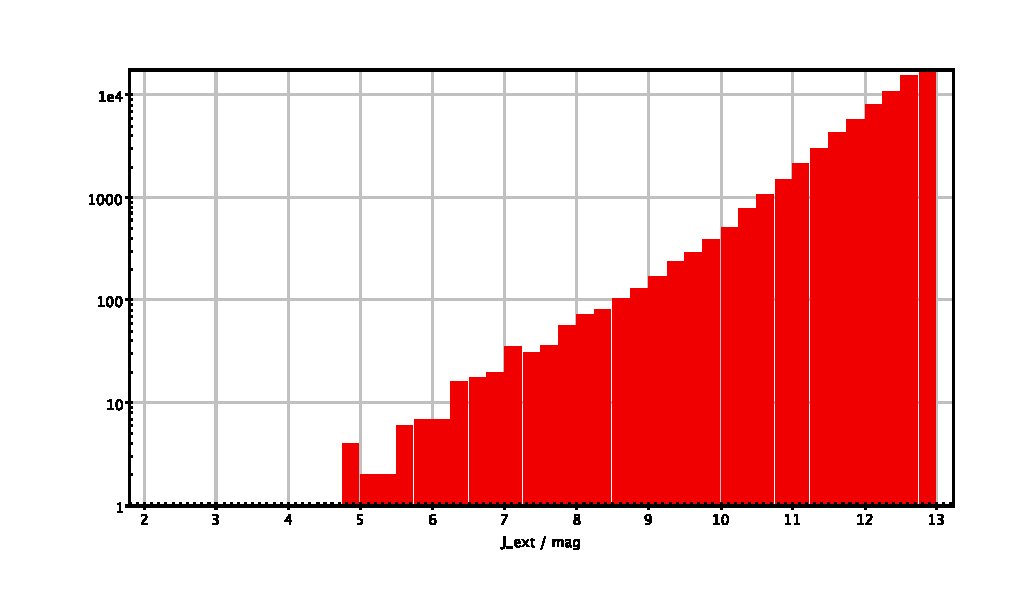
\includegraphics[width=.9\textwidth]{./2MASX.eps}
\caption{2MASX}
\label{fig:3}
\end{figure}
The slope was calculated as:
\begin{equation}
\frac{log(10000/1000)}{12/11}=.9
\end{equation}
This is a similar figure to the 2MRS survey.

\section{}
Figure 4 shows the 2MRS data in galactic coordinates restricted to the the closest half of the galaxies i.e. $cz<8000$ km/s.
It clearly shows evidence of structure indicating that the universe is not homogeneous on smaller scales.
\begin{figure}[H]
\centering
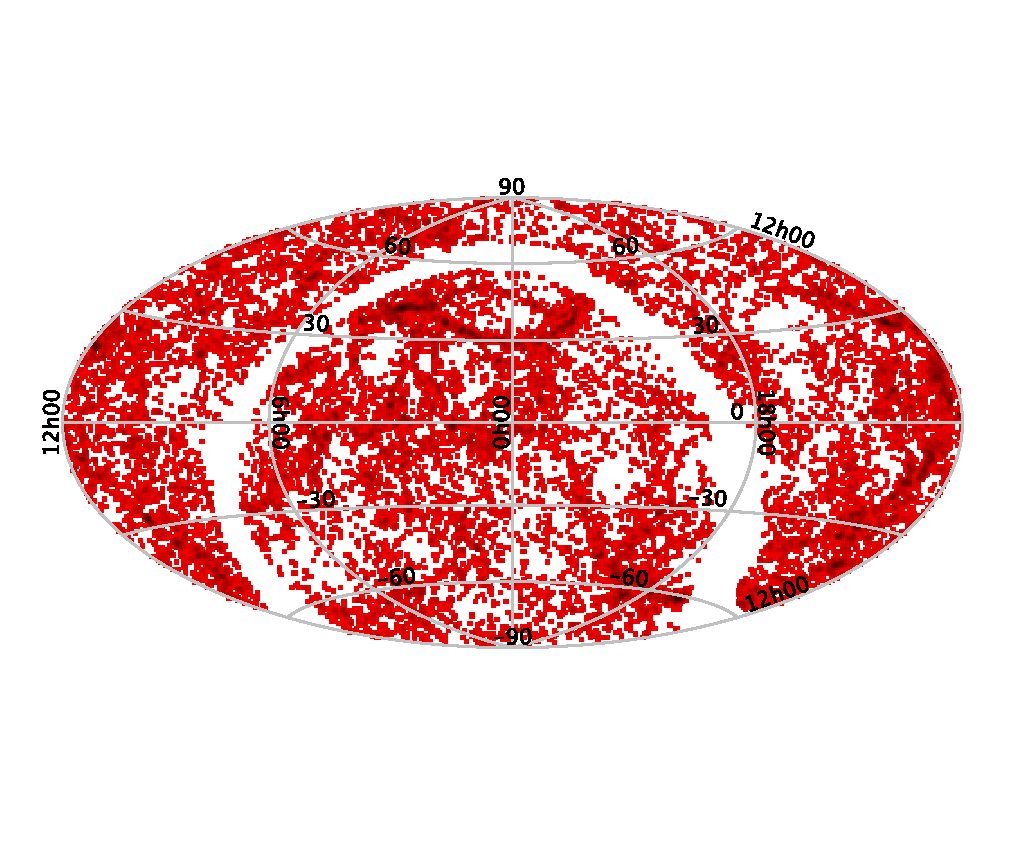
\includegraphics[width=.9\textwidth]{./NearestGalaxies.eps}
\caption{2MRS}
\label{fig:4}
\end{figure}


%\begin{thebibliography}{1}
%\end{thebibliography}
\end{document} 